\scanpage{28}
\mspage{27}
% Reused typed sheet, read after rotation through 180 degrees.
\begin{center}-2.14-\end{center}

is still closed. Therefore, by definition, $x$ is a point of $\mathcal U$.

Therefore, a quasi-projective geometric quotient $X/\mathbb G_m$ exists. But this implies that the action of $\mathbb G_m$ on $X$ is separated. Therefore, by lemma 0.5, the action of $\mathbb G_m$ on $X$ is proper. \uline{QED}

\figure{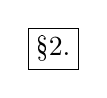
\begin{tikzpicture}[baseline=(heading.base)]\node[draw,inner sep=3pt] (heading) {\S 2.};\end{tikzpicture}} In the last section, we have related the concept of stability with respect to actions of $G$ to the function $\mu^L(x;\lambda)$ involving a 1-parameter subgroup $\lambda$ of $G$. In this section, we shall consider the dependence of $\mu$ on $\lambda$. The analysis leads naturally to an ungainly but remarkable metric space investigated extensively by J. Tits, which we will call the \uline{flag complex} of $G$. The first step is:

\uline{Definition 2.3}/\uline{Proposition 2.6}: Let $G$ be a reductive algebraic group and let $\lambda$ be a 1-PS of $G$. Then there is a unique algebraic subgroup $P(\lambda)\subset G$ such that:
\[
\begin{aligned}
\gamma\in P(\lambda)_k\quad\Longleftrightarrow\quad&
\lambda(\alpha)\cdot\gamma\cdot\lambda(\alpha^{-1})\quad\text{has a specialization in }G\\
&\text{when }\alpha\in(\mathbb G_m)_k\text{ specializes to }0.
\end{aligned}
\]
Moreover, $P(\lambda)$ is a parabolic subgroup of $G$, $\lambda$ is a 1-PS of the radical of $P(\lambda)$, and the specialization $\gamma'$ of $\lambda(\alpha)\cdot\gamma\cdot\lambda(\alpha^{-1})$, as $\alpha\longrightarrow0$, centralizes $\lambda$.

\uline{Proof}: Most of these facts can be seen most easily by means of a faithful representation $\phi:G\longrightarrow\mathrm{GL}(n)$. Recall that the image $\phi(G)$ is \uline{closed} in $\mathrm{GL}(n)$. Therefore, $P(\lambda)=\phi^{-1}(P(\phi\circ\lambda))$, at least as a set of closed points. Now by composing $\phi$ \deleted{$\unsure{\Rightarrow}$}\inserted{with} a suitable inner automorphism of $\mathrm{GL}(n)$, we may assume that $\phi\circ\lambda$ is diagonalized, i.e.
